\chapter{Analisis Masalah dan Perancangan Solusi}

Bab ini memaparkan skema penelitian yang dilakukan untuk menjawab persoalan yang dibahas pada Bab I.

\section{Analisis Permasalahan}

Ada beberapa permasalahan yang ditemukan pada permasalahan pengenalan ucapan, dan salah satunya dan yang menjadi fokus pada penelitian ini adalah kesulitan sistem pengenal ucapan dalam mengenali suara pada lingkungan yang bising. Beberapa penelitian-penelitian terkait mengenai permasalahan tersebut mencoba untuk menyelesaikannya dengan menambahkan informasi visual pada proses pengenalan suaranya, seperti pada penelitian \textcite{Chung2017}, \textcite{Chung2016}, dan \textcite{Assael2016}.
\bigskip

Untuk penelitian-penelitian mengenai pengenalan ucapan untuk bahasa Indonesia sejauh ini sudah banyak yang menggunakan pendekatan \textit{deep learning}, seperti pada penelitian \textcite{Yuwan2018} yang membangun model akustik ucapan spontan bahasa Indonesia berbasis DNN-HMM, akan tetapi belum ada penelitian yang menggabungkan fitur akustik dan fitur visual, baik yang menggunakan fitur \textit{handcrafted} dan model akustik berbasis statistik maupun \textit{deep learning}.
\bigskip

Fitur visual yang digunakan dalam mengenali ucapan adalah berupa informasi gerak bibir, seperti yang biasa dilakukan oleh manusia. Penelitian-penelitian terkait pembacaan gerak bibir untuk bahasa Indonesia masih terbilang sedikit jika dibandingkan dengan penelitian-penelitian terkait untuk bahasa lain, terutama bahasa Inggris. Penelitian mengenai pembacaan gerak bibir yang menggunakan dataset bahasa Indonesia kebanyakan masih belum menggunakan \textit{deep learning}, seperti pada penelitian \textcite{Achmad2015} yang menggunakan HMM menunjukkan bahwa hasil pengenalan masih belum tergeneralisasi dengan baik karena hasilnya masih berpengaruh pada kondisi bibir pembicara, yang dalam hal ini pembicara wanita dengan bibir yang menggunakan lipstik memiliki koefisien korelasi yang tinggi sedangkan untuk yang bibir berwarna pucat dan bibir yang memiliki kumis di atasnya memiliki koefisien korelasi yang rendah.
\bigskip

Selain penelitian tersebut, pada saat penulisan, hanya ada satu penelitian mengenai pembacaan gerak bibir dalam bahasa Indonesia yang menggunakan pendekatan \textit{deep learning}, yaitu oleh \textcite{Maulana2017}, yang menggunakan \textit{spatiotemporal} CNN untuk menangkap struktur \textit{spatiotemporal} dari video, dan menggunakan \textit{bidirectional} Gated Recurrent Unit (GRU) untuk memodelkan keseluruhan rangkaian frame video dari dua arah, baik dengan urutan frame normal maupun dengan urutan terbalik. Kinerjanya sudah sangat baik, dengan WER 13.3\% dan BLEU 90.4\% untuk model yang dilatih menggunakan pembicara-pembicara yang tidak ada di data uji, dan WER 8.0\% dan BLEU 94.7\% untuk model yang dilatih menggunakan pembicara-pembicara yang ada di data uji. Akan tetapi data yang digunakan adalah data AVID, yang merupakan versi bahasa Indonesia dari dataset GRID. Dataset GRID itu sendiri terdiri atas kalimat-kalimat berstruktur \textit{command} + \textit{color} + \textit{preposition} + \textit{letter} + \textit{digit} + \textit{adverb} dan kosakata yang terbatas, dibandingkan dengan dataset LRW yang memiliki kosakata terbuka. Jika dibandingkan dengan penelitian \textcite{Chung2016} untuk pengenalan dalam bahasa Inggris, model \textit{sequence-to-sequence}nya berhasil mencapai kinerja WER 3.0\% untuk dataset GRID, tetapi untuk dataset LRW hanya mencapai WER 23.8\%, sehingga masih ada ruang untuk perbaikan, baik untuk bahasa Indonesia maupun bahasa Inggris.
\bigskip

Salah satu permasalahan yang ditemui dalam penggunaan model \textit{sequence-to-sequence} untuk mentransduksi sebuah rangkaian menjadi rangkaian lain adalah kebanyakan model ini menggunakan RNN atau variannya sehingga prosesnya tidak bisa diparalelisasi karena sifatnya yang rekurens. Oleh sebab itu, proses pelatihan model membutuhkan waktu yang lama hingga model akhirnya konvergen. Pada penelitian \textcite{Vaswani2017} diusulkan model yang disebut sebagai model transformer, sebuah arsitektur model yang menghindari penggunaan rekurens dan bergantung sepenuhnya pada mekanisme \textit{attention} untuk menggambarkan dependensi global antara masukan dan keluaran. Selain itu model transformer ini memungkinkan dilakukannya paralelisasi sehingga dapat mempercepat proses pelatihan model, dan juga berhasil mengungguli model \textit{encoder-decoder} berbasis RNN dalam mentransduksi rangkaian.


\section{Analisis Solusi}

Berdasarkan ulasan masalah yang dipaparkan pada subbab III.1, penelitian ini akan membangun solusi pemodelan akustik dan visual menggunakan model transformer. Agar diketahui peningkatan kinerja AVSR yang menggunakan model transformer, diimplementasikan juga model \textit{sequence-to-sequence} dari \textcite{Chung2017} sebagai model tolok ukur. Selain itu dibangun juga solusi pemodelan dengan berbasis akustik saja, dan juga pemodelan dengan berbasis visual saja, untuk melihat peningkatan kinerja ASR setelah penambahan fitur visual.


\subsection{Persiapan Korpus Video}
\label{subsec:korpus}

Korpus video diperoleh dari data yang digunakan pada penelitian sebelumnya \textcite{Chung2017}. Korpus video tersebut terdiri atas tiga jenis korpus, yaitu LRW, LRS2, dan LRS3. Untuk korpus LRW dan LRS2 bersumber dari televisi BBC UK sehingga untuk perolehan korpus tersebut sedikit dipersulit sehingga hanya digunakan korpus LRS3 saja yang bersumber dari TED. Ketiga korpus tersebut merupakan korpus dalam bahasa Inggris dan digunakan untuk pelatihan model awal. Selanjutnya dilakukan \textit{transfer learning} dan model selanjutnya dilatih menggunakan korpus bahasa Indonesia. korpus bahasa Indonesia ini dikumpulkan dari situs YouTube berisi pembicara-pembicara di TEDxJakarta dan BukaTalks, dengan total durasi video adalah 10 jam. Untuk korpus LRS3 berdurasi sekitar 800 jam dan memuat 150 ribu kalimat atau sekitar 50 ribu kosakata.

\subsection{Pengenalan Wajah}

Untuk bagian video, sebelum masuk ke dalam model transformer, setiap framenya akan melalui tahap pengenalan wajah terlebih dahulu untuk diketahui apakah frame tersebut terdapat wajah manusia atau tidak, lalu kemudian jika ditemukan wajah maka akan dicari \textit{landmark} pada wajah tersebut, sehingga dapat diketahui letak bibir pada wajah tersebut. Tahap pengenalan wajah ini dilakukan dengan menggunakan \textit{library} OpenFace. OpenFace merupakan \textit{library} Python dan Torch dalam mengimplementasikan modul pengenalan wajah yang menggunakan algoritma DNN (\textit{deep neural network}). Torch mendukung agar OpenFace dapat dieksekusi dengan menggunakan CPU maupun dengan menggunakan GPU (dalam hal ini menggunakan CUDA). OpenFace menggunakan beberapa \textit{library} pendukung yakni dlib dan OpenCV.

\begin{figure}[h]
    \centering
    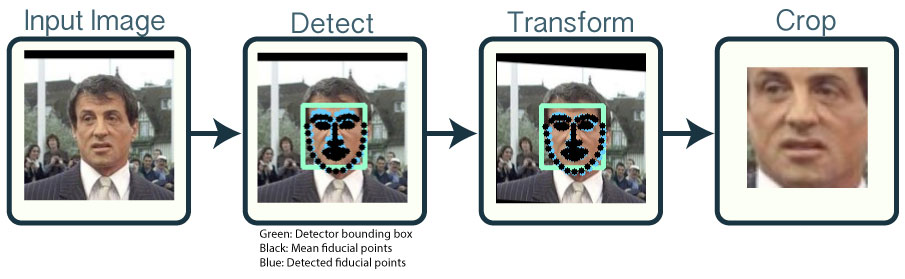
\includegraphics[width=0.8\textwidth]{resources/images/arsitektur-openface.png}
    \caption{Alur pengenalan wajah pada OpenFace.}
    \label{fig:arsitektur-openface}
\end{figure}


\subsection{Pembangunan Kamus Pelafalan}

Kamus pelafalan dibangun dengan cara memetakan setiap kata yang ada pada corpus ke dalam fonem bahasa Indonesia. Fonem bahasa Indonesia tersebut seluruhnya didaftarkan sebagai fonem penyusun leksikon. Pada penelitian ini kamus pelafalan dibangun dengan menggunakan kakas Corpus Management Tools, yang dikembangkan oleh Hoesen (2015). Kakas bekerja dengan cara mengolah teks masukan kemudian membangun skema pelafalan kata bahasa Indonesia berdasarkan aspek fonetis.


\subsection{Rancangan Arsitektur}

\begin{figure}[h]
    \centering
    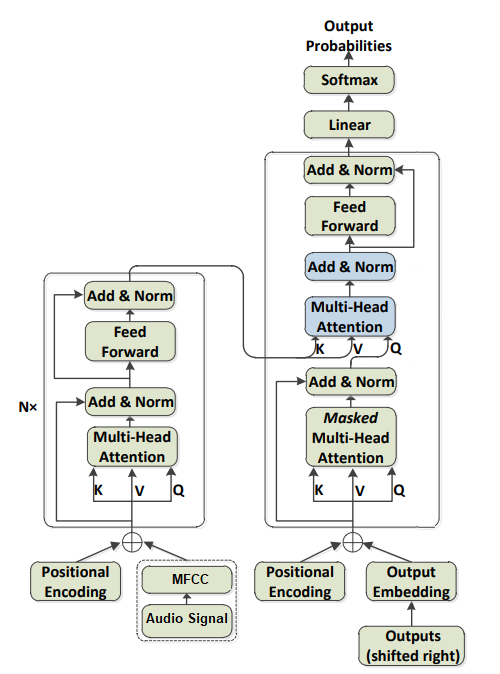
\includegraphics[width=0.8\textwidth]{resources/images/usulan-arsitektur-asr.png}
    \caption{Rancangan Arsitektur ASR.}
    \label{fig:usulan-arsitektur-asr}
\end{figure}

\begin{figure}[h]
    \centering
    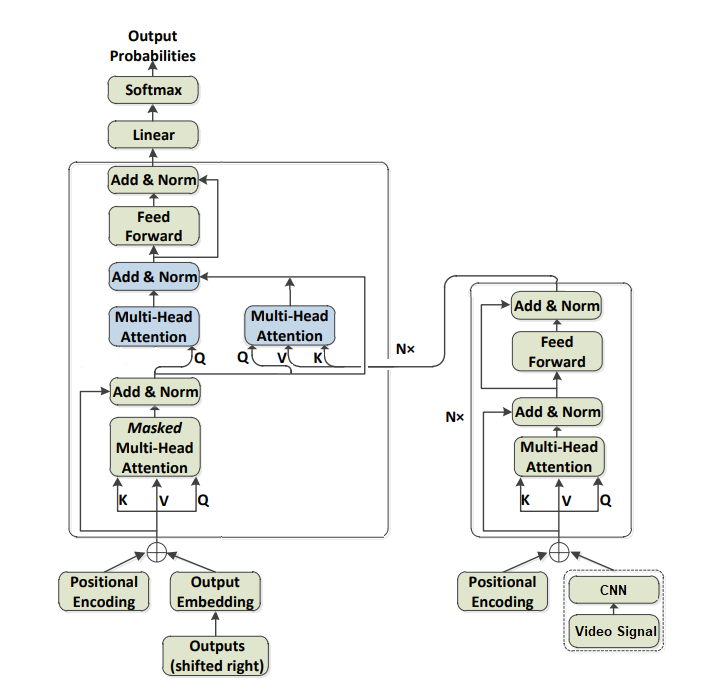
\includegraphics[width=0.8\textwidth]{resources/images/usulan-arsitektur-vsr.png}
    \caption{Rancangan Arsitektur VSR.}
    \label{fig:usulan-arsitektur-vsr}
\end{figure}

\begin{figure}[h]
    \centering
    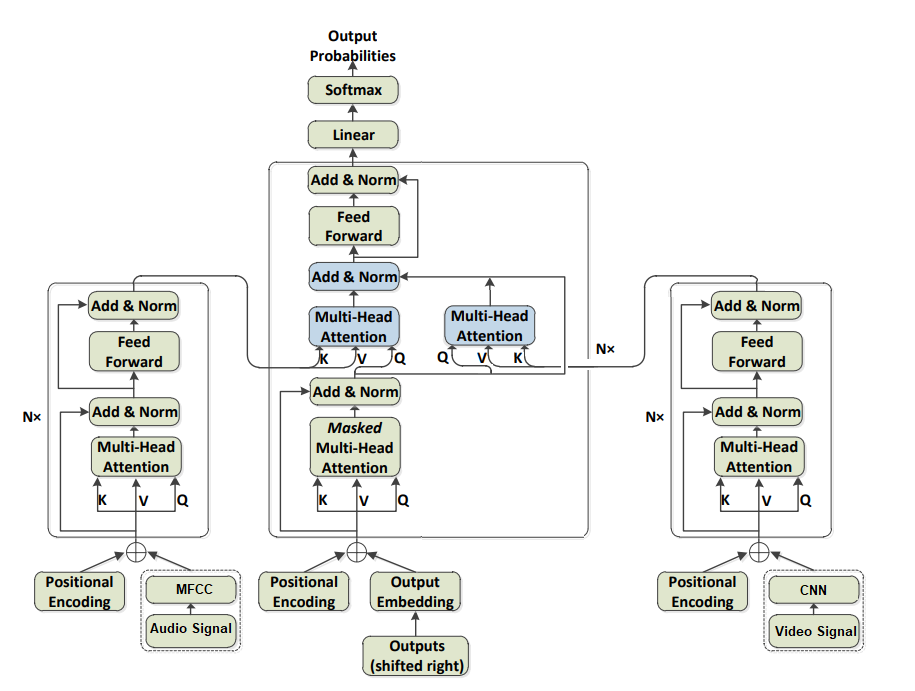
\includegraphics[width=0.8\textwidth]{resources/images/usulan-arsitektur-avsr.png}
    \caption{Rancangan Arsitektur AVSR.}
    \label{fig:usulan-arsitektur-avsr}
\end{figure}

Pada bagian ini dijelaskan rancangan arsitektur untuk proses pengenalan ucapan. Rancangan model arsitektur yang diusulkan dibagi menjadi tiga model, yaitu:
\begin{enumerate}
    \item model yang menggunakan modal akustik saja. Model ini menggunakan arsitektur transformer (Gambar \ref{fig:usulan-arsitektur-asr}) dan dilakukan pelatihan menggunakan dataset yang sudah dijelaskan pada upabab \ref{subsec:korpus}. Masukan dari dataset tersebut berupa \textit{raw speech} yang kemudian diekstraksi fiturnya dengan menggunakan MFCC. Selanjutnya model ini akan disebut sebagai model transASR.
    \item model yang menggunakan modal visual saja. Model ini menggunakan arsitektur transformer (Gambar \ref{fig:usulan-arsitektur-vsr}) dan dilakukan pelatihan menggunakan dataset yang sudah dijelaskan pada upabab \ref{subsec:korpus}. Masukan berupa frame video yang direpresentasikan menjadi vektor berukuran tetap menggunakan arsitektur CNN yang belum ditentukan. Untuk selanjutnya model ini akan disebut sebagai model transVSR.
    \item terakhir adalah model yang menggunakan modal akustik dan modal visual secara bersamaan. Model ini juga menggunakan arsitektur transformer (Gambar \ref{fig:usulan-arsitektur-avsr}) dan dilakukan pelatihan menggunakan dataset yang sudah dijelaskan pada upabab \ref{subsec:korpus}. Masukan berupa \textit{raw speech} dan frame video. Selanjutnya model ini akan disebut sebagai model transAVSR.
\end{enumerate}

% penjelasan komponen-komponennya jelasin kalo ada di bab 2 %
Selain frame video dan \textit{raw speech}, terdapat juga masukan berupa keluaran-keluaran sebelumnya dari model, sehingga keluaran dari time-step saat ini akan digunakan juga untuk masukan di time-step selanjutnya.
\bigskip

Komponen-komponen pembentuk dari model transformer itu sendiri adalah komponen \textit{positional encoding}, \textit{multi-head attention}, dan \textit{masked multi-head attention}, yang sudah dijelaskan sebelumnya pada upabab \ref{subsec:encoder-decoder-attention}.

\subsection{Evaluasi Sistem}

% tambahin CER, penjelasan WER, dan BLEU, rumus2nya %
Kinerja dari sistem diukur dengan menggunakan tiga metrik pengujian yang umum digunakan pada kasus penganalan ucapan dan translasi, yaitu \textit{character error rate} (CER), \textit{word error rate} (WER), dan \textit{bilingual evaluation understudy} (BLEU). WER dan CER dihitung dengan menggunakan rumus:

\begin{equation*}
    \begin{split}
        WER &= 100 \times \frac{S + D + I}{N} \\
        &= 100 \times \frac{S + D + I}{S + D + C}
    \end{split}
\end{equation*}

yang dalam hal ini, \(S\) merupakan jumlah substitusi kata (untuk WER) atau karakter (untuk CER) yang dikenali, \(D\) merupakan jumlah penghapusan kata atau karakter, \(I\) merupakan jumlah penyisipan kata atau karakter, \(C\) merupakan jumlah kata atau karakter yang benar, dan \(N\) adalah jumlah keseluruhan kata atau karakter yang ada pada transkripsi. Semakin kecil nilai WER dan CER maka semakin semakin baik kinerja model dalam mengenali ucapan.
\bigskip

BLEU merupakan presisi n-gram yang telah dimodifikasi dan digunakan untuk membandingkan kalimat yang dihasilkan sistem dengan kalimat yang ada di transkripsi. BLEU dihitung dengan menggunakan persamaan berikut.

\begin{equation*}
    \begin{split}
        P &= \frac{m}{w_t}\\
        p &= \begin{cases}
            1                      & jika \quad c>r \\
            e^{(1-\frac{r}{c})}    & jika \quad c \leq r
        \end{cases} \\
        BLEU &= p \times e^{\sum_{n=1}^{N} (\frac{1}{N}\times log Pn)}
    \end{split}
\end{equation*}

yang dalam hal ini \(P\) merupakan presisi unigram, \(p\) merupakan \textit{brevity penalty} atau penalti jika kalimat yang dihasilkan lebih pendek dari kalimat yang ada di transkripsi, \(r\) adalah panjang efektif dari kalimat di transkripsi, dan \(c\) merupakan total panjang keseluruhan kalimat yang dihasilkan sistem. Jenis BLEU yang akan digunakan dalam evaluasi ini adalah unigram BLEU.

Pengujian dilakukan dengan membandingkan kegita model yang telah dibuat (transASR, transVSR, dan transAVSR).